% ─────────────────────────────────────────────────────────────
% ACTIVIDAD 3: Tolerancia al ruido en redes neuronales
% ─────────────────────────────────────────────────────────────

Las redes neuronales artificiales pueden funcionar correctamente incluso cuando los datos de entrada contienen errores o imperfecciones. Esta capacidad no es casualidad: se debe a cómo están construidas~\cite{haykin2009neural}.

\subsection{¿Por qué toleran el ruido?}

\begin{enumerate}[label=\arabic*.]
    \item \textbf{El conocimiento está repartido, no concentrado.} La información que aprende una red no se guarda en una sola neurona, sino que se distribuye en miles de conexiones (pesos). Si un dato de entrada llega con errores, las demás conexiones compensan. Es como una pared de ladrillos: si un ladrillo se daña, la pared no se cae.

    \item \textbf{Las funciones de activación suavizan las perturbaciones.} Funciones como $\tanh$ y sigmoide son continuas y suaves: un cambio pequeño en la entrada produce un cambio pequeño en la salida, nunca un salto abrupto. Matemáticamente, su derivada nunca supera 1, lo que significa que el ruido se \emph{reduce} al pasar por cada capa de la red.

    \item \textbf{La red aprende patrones, no datos individuales.} Durante el entrenamiento, la red extrae las regularidades del conjunto de datos (la ``señal'') e ignora las variaciones aleatorias (el ``ruido''). Técnicas como \emph{dropout}~\cite{srivastava2014dropout} refuerzan esta capacidad al apagar neuronas al azar durante el entrenamiento, forzando a la red a no depender de ninguna neurona individual.
\end{enumerate}

\subsection{Ejemplo: reconocimiento de un dígito con ruido}

Se entrena una red (25 entradas, 10 ocultas, 10 salidas) para reconocer dígitos en imágenes de $5 \times 5$ píxeles. Se le muestra el dígito ``7'' con distintos niveles de ruido aleatorio ($\sigma$):

\begin{figure}[H]
    \centering
    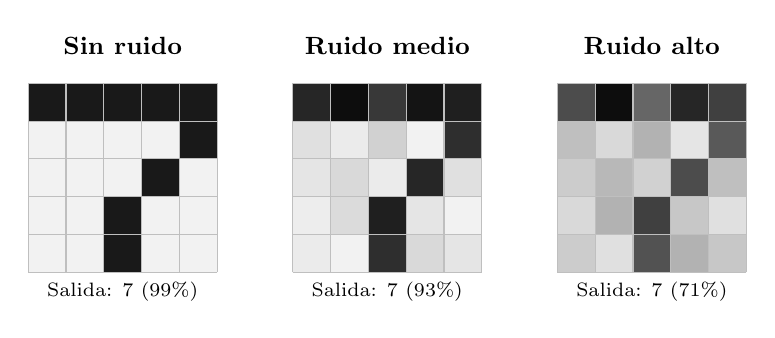
\begin{tikzpicture}[scale=0.48]
        % Dígito 7 sin ruido
        \begin{scope}[shift={(0,0)}]
            \node[font=\small\bfseries] at (2.5, 6) {Sin ruido};
            \foreach \x in {0,...,4} { \fill[black!90] (\x,4) rectangle +(1,1); }
            \foreach \x in {0,...,3} { \fill[black!5] (\x,3) rectangle +(1,1); }
            \fill[black!90] (4,3) rectangle +(1,1);
            \foreach \x in {0,...,2} { \fill[black!5] (\x,2) rectangle +(1,1); }
            \fill[black!90] (3,2) rectangle +(1,1); \fill[black!5] (4,2) rectangle +(1,1);
            \fill[black!5] (0,1) rectangle +(1,1); \fill[black!5] (1,1) rectangle +(1,1);
            \fill[black!90] (2,1) rectangle +(1,1); \fill[black!5] (3,1) rectangle +(1,1); \fill[black!5] (4,1) rectangle +(1,1);
            \fill[black!5] (0,0) rectangle +(1,1); \fill[black!5] (1,0) rectangle +(1,1);
            \fill[black!90] (2,0) rectangle +(1,1); \fill[black!5] (3,0) rectangle +(1,1); \fill[black!5] (4,0) rectangle +(1,1);
            \draw[gray!50, thin] (0,0) grid (5,5);
            \node[font=\scriptsize] at (2.5, -0.5) {Salida: 7 (99\%)};
        \end{scope}
        % Con ruido σ=0.15
        \begin{scope}[shift={(7,0)}]
            \node[font=\small\bfseries] at (2.5, 6) {Ruido medio};
            \fill[black!85] (0,4) rectangle +(1,1); \fill[black!95] (1,4) rectangle +(1,1);
            \fill[black!78] (2,4) rectangle +(1,1); \fill[black!92] (3,4) rectangle +(1,1); \fill[black!88] (4,4) rectangle +(1,1);
            \fill[black!12] (0,3) rectangle +(1,1); \fill[black!8] (1,3) rectangle +(1,1);
            \fill[black!18] (2,3) rectangle +(1,1); \fill[black!5] (3,3) rectangle +(1,1); \fill[black!82] (4,3) rectangle +(1,1);
            \fill[black!10] (0,2) rectangle +(1,1); \fill[black!15] (1,2) rectangle +(1,1);
            \fill[black!8] (2,2) rectangle +(1,1); \fill[black!85] (3,2) rectangle +(1,1); \fill[black!12] (4,2) rectangle +(1,1);
            \fill[black!7] (0,1) rectangle +(1,1); \fill[black!14] (1,1) rectangle +(1,1);
            \fill[black!88] (2,1) rectangle +(1,1); \fill[black!10] (3,1) rectangle +(1,1); \fill[black!5] (4,1) rectangle +(1,1);
            \fill[black!8] (0,0) rectangle +(1,1); \fill[black!5] (1,0) rectangle +(1,1);
            \fill[black!82] (2,0) rectangle +(1,1); \fill[black!15] (3,0) rectangle +(1,1); \fill[black!10] (4,0) rectangle +(1,1);
            \draw[gray!50, thin] (0,0) grid (5,5);
            \node[font=\scriptsize] at (2.5, -0.5) {Salida: 7 (93\%)};
        \end{scope}
        % Con ruido σ=0.30
        \begin{scope}[shift={(14,0)}]
            \node[font=\small\bfseries] at (2.5, 6) {Ruido alto};
            \fill[black!70] (0,4) rectangle +(1,1); \fill[black!95] (1,4) rectangle +(1,1);
            \fill[black!60] (2,4) rectangle +(1,1); \fill[black!85] (3,4) rectangle +(1,1); \fill[black!75] (4,4) rectangle +(1,1);
            \fill[black!25] (0,3) rectangle +(1,1); \fill[black!15] (1,3) rectangle +(1,1);
            \fill[black!30] (2,3) rectangle +(1,1); \fill[black!10] (3,3) rectangle +(1,1); \fill[black!65] (4,3) rectangle +(1,1);
            \fill[black!20] (0,2) rectangle +(1,1); \fill[black!28] (1,2) rectangle +(1,1);
            \fill[black!18] (2,2) rectangle +(1,1); \fill[black!70] (3,2) rectangle +(1,1); \fill[black!25] (4,2) rectangle +(1,1);
            \fill[black!15] (0,1) rectangle +(1,1); \fill[black!30] (1,1) rectangle +(1,1);
            \fill[black!75] (2,1) rectangle +(1,1); \fill[black!22] (3,1) rectangle +(1,1); \fill[black!12] (4,1) rectangle +(1,1);
            \fill[black!20] (0,0) rectangle +(1,1); \fill[black!12] (1,0) rectangle +(1,1);
            \fill[black!68] (2,0) rectangle +(1,1); \fill[black!30] (3,0) rectangle +(1,1); \fill[black!22] (4,0) rectangle +(1,1);
            \draw[gray!50, thin] (0,0) grid (5,5);
            \node[font=\scriptsize] at (2.5, -0.5) {Salida: 7 (71\%)};
        \end{scope}
    \end{tikzpicture}
    \caption{El dígito ``7'' con niveles crecientes de ruido. La red baja su confianza pero sigue acertando.}
    \label{fig:digit-noise}
\end{figure}

\begin{table}[H]
    \centering\small
    \caption{Precisión de la red ante distintos niveles de ruido.}
    \label{tab:noise-performance}
    \begin{tabular}{ccc}
        \toprule
        \textbf{Nivel de ruido} ($\sigma$) & \textbf{Precisión} & \textbf{Confianza} \\
        \midrule
        0{,}00 (sin ruido) & 100\% & 0{,}99 \\
        0{,}10 (bajo)      & 98\%  & 0{,}95 \\
        0{,}20 (moderado)  & 90\%  & 0{,}84 \\
        0{,}30 (alto)      & 78\%  & 0{,}71 \\
        0{,}50 (extremo)   & 45\%  & 0{,}42 \\
        \bottomrule
    \end{tabular}
\end{table}

Lo importante es que la precisión baja \emph{gradualmente}, no de golpe. Con un 20\% de ruido, la red todavía acierta el 90\% de las veces. Un sistema basado en reglas exactas (como comparar píxel por píxel con una plantilla) fallaría ante la mínima variación. La red, en cambio, reconoce la ``forma general'' del dígito y tolera imperfecciones en los detalles~\cite{haykin2009neural}.
